\documentclass[12pt,fleqn]{article}\usepackage{../../common}
\begin{document}
Bir ODE Sistemi Sayısal Olarak Nasıl Çözülür

Yazıda \verb!scipy! paketinin içindeki \verb!odeint! çözücüyü işleyeceğiz.
Sayısal çözümler önemli çünkü çoğu ODE sisteminin analitik çözümü
yoktur. Onları sayısal paketler kullanarak çözmek gerekir. 

Bir sarkaç denklemi düşünelim, bu denklem ikinci dereceden $\theta$'yi baz
alan bir denklemdir,

$$
\ddot{\theta}(t) + \frac{b}{m} \dot{\theta}(t) +  \frac{g}{L} \sin(\theta(t)) = 0
$$

Ya da $m = 1$ dersek ve $\frac{g}{L} = c$ ile

$$
\ddot{\theta}(t) + b \dot{\theta}(t) +  c \sin(\theta(t)) = 0
$$

ki $b,c$ dışarıdan tanımlanan sabitler, ve üst nokta zamansal türevi temsil
ediyor. 

Bu denklemi \verb!odeint! ile çözmek için onu ilk önce bir birinci derece
denklemler sistemine çevirmemiz gerekiyor.

$$
\omega(t) = \dot{\theta}(t)
$$

dersek (okunuş olarak $\omega$ omega, $\theta$ theta),

$$
\dot{\theta} = \omega(t)
$$

$$
\dot{\omega}(t) = -b \omega(t) - c\sin(\theta(t))
$$

elde ederiz. Şimdi \verb!pend! adlı bir fonksiyon tanımlayalım,

\begin{minted}[fontsize=\footnotesize]{python}
b = 0.25
c = 5.0

def pend(y, t):
    theta, omega = y
    return [omega, -b*omega - c*np.sin(theta)]
\end{minted}

Bu fonksiyon ana ODE çözücünün denklemimiz hakkında bilgi aldığı nokta,
\verb!y! dizini içinde $\dot{\theta}$ ve $\dot{\omega}$ var, onları $y$
içinde aynen bu sırada almayı bekliyoruz ve yenilerini hesapladıktan sonra
geri döndürürken de aynen bu sırada döndürüyoruz. Mesela döndürülen dizinde
ilk öğe \verb!omega! var, bu doğru, çünkü biraz önce
$\dot{\theta} = \omega(t)$ tanımını yapmıştık, yani ilk öğede \verb!theta!
turevi geri vermiş olduk, alırken \verb!theta,omega=y! ile \verb!theta!
aldığımız gibi.

\verb!t! değişkeninde çoğunlukla zaman tanımlanır, ve bu zaman
ilgilendiğimiz zaman aralığı belli (çoğunlukla eşit aralıklı) noktalar
üzerinden dizin olarak \verb!odeint!'e verilir, bunu \verb!linspace! ile
yapabiliriz. $y$ için başlangıç şartlarını ayrı bir değişken içinde, mesela
\verb!y0!, tanımlarız, bu aynen \verb!y! büyüklüğünde bir dizin olacaktır
ve \verb!y!  için olduğu gibi ilk öğe \verb!theta! ikinci öğe \verb!omega!
için başlangıç değerini tanımlayacak.

Hepsi bir arada

\begin{minted}[fontsize=\footnotesize]{python}
from scipy.integrate import odeint

b = 0.25
c = 5.0

def pend(y, t):
    theta, omega = y
    return [omega, -b*omega - c*np.sin(theta)]

t = np.linspace(0, 10, 101)

y0 = [np.pi - 0.1, 0.0]

sol = odeint(pend, y0, t)

print (sol.shape)
\end{minted}

\begin{verbatim}
(101, 2)
\end{verbatim}

Başlangıç noktası $\theta$ için $\pi - 0.1$, yani şarkacın en üst
noktasından biraz yanda. Açı olarak $\theta=0$ sarkacın nötr durduğu nokta,
$\pi$ en üst noktası.

Sayısal çözüm sırasında bir dizi $\theta,\omega$ elde edildi. Bu değerler
hesaplandıkları gibi zamansal sırada, bir dizin içindeler ve üstte
gördüğümüz gibi \verb!101,2! boyutlu bir dizin bu. En son varılan değer

\begin{minted}[fontsize=\footnotesize]{python}
print (sol[-1])
\end{minted}

\begin{verbatim}
[0.02001168 1.56781812]
\end{verbatim}

Degiskenleri grafiklersek

\begin{minted}[fontsize=\footnotesize]{python}
import matplotlib.pyplot as plt
plt.plot(t, sol[:, 0], 'b', label='theta(t)')
plt.plot(t, sol[:, 1], 'g', label='omega(t)')
plt.legend(loc='best')
plt.xlabel('t')
plt.grid()
plt.savefig('ode_mattuck_70_odeint_01.png')
\end{minted}

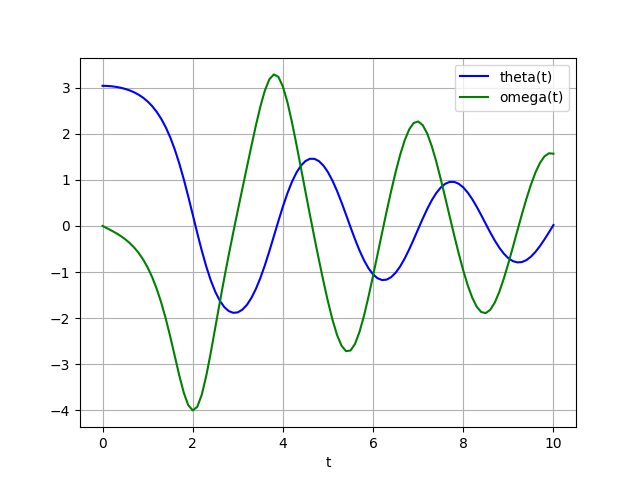
\includegraphics[height=6cm]{ode_mattuck_70_odeint_01.png}

Şarkaçın hareketini görmek istiyorsak,

\begin{minted}[fontsize=\footnotesize]{python}
L = 9.8 / c
x1 = L*np.sin(sol[:,0])
y1 = -L*np.cos(sol[:,0])
\end{minted}

\begin{minted}[fontsize=\footnotesize]{python}
from matplotlib.patches import Circle
import matplotlib.pyplot as plt
from numpy import cos, sin

def make_plot(fout,x1,y1):
    r = 0.05
    fig = plt.figure()
    ax = fig.add_subplot(111)
    ax.set_xlim(-3,3)
    ax.set_ylim(-3,3)
    plt.plot([0, x1], [0, y1], lw=2, c='k')
    c0 = Circle((0, 0), r/2, fc='k', zorder=10)
    c1 = Circle((x1, y1), r, fc='b', ec='b', zorder=10)
    ax.add_patch(c0)
    ax.add_patch(c1)
    plt.savefig(fout)

for i in range(len(x1)):
    if i % 5 == 0: 
        make_plot('frames/img{:04d}.png'.format(i),x1[i],y1[i])
\end{minted}

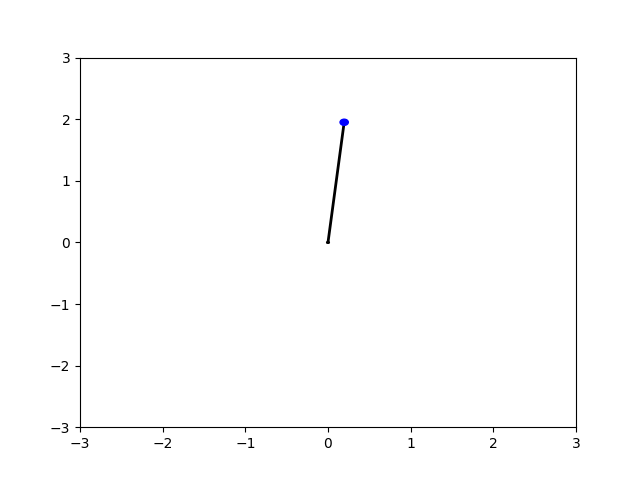
\includegraphics[width=12em]{frames/img0000.png}
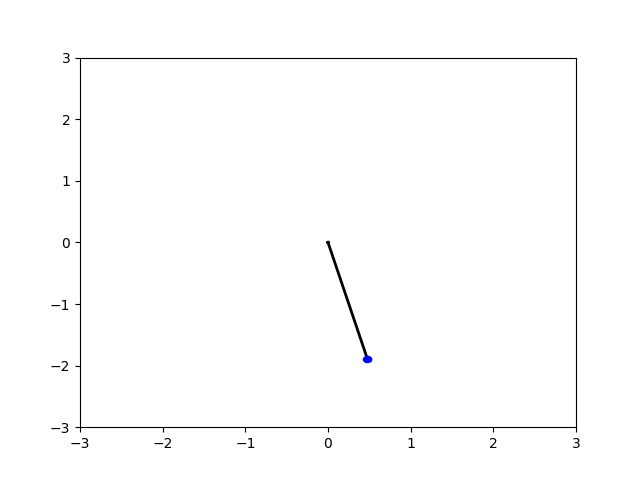
\includegraphics[width=12em]{frames/img0020.png}
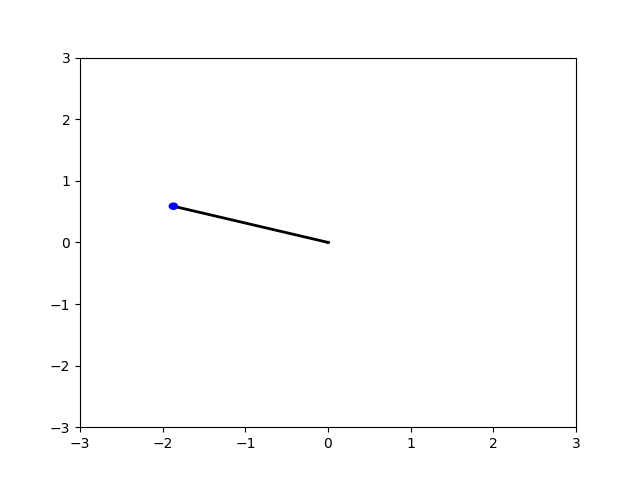
\includegraphics[width=12em]{frames/img0030.png}
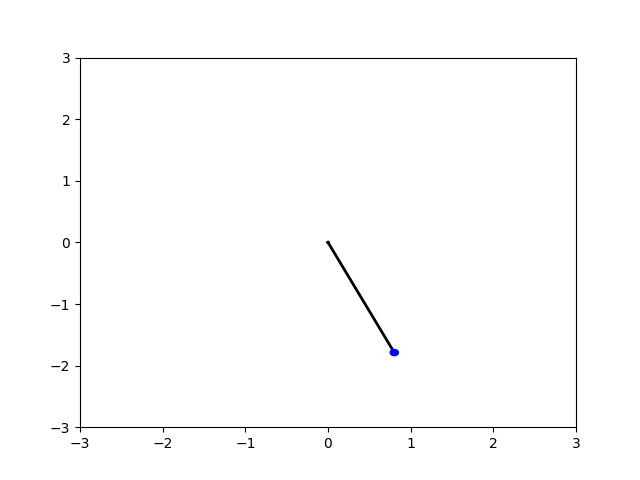
\includegraphics[width=12em]{frames/img0040.png}
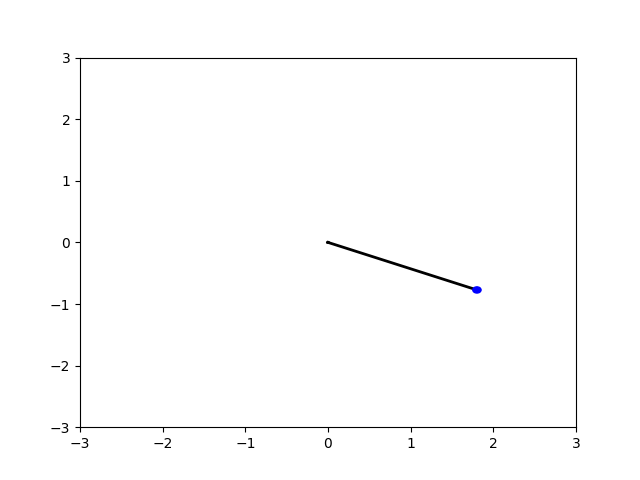
\includegraphics[width=12em]{frames/img0050.png}
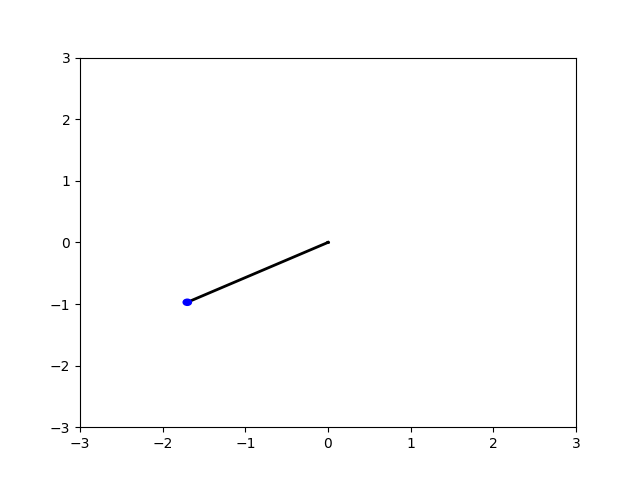
\includegraphics[width=12em]{frames/img0060.png}

Animasyon yaratabiliriz,

\begin{minted}[fontsize=\footnotesize]{python}
! convert -loop 0 -delay 100 frames/*.png frames/pend.gif
\end{minted}

Sonuç [2]'de görülebilir.

Not: Bir ODE sistemini çözmek hakkında konuşurken bazen onu ``entegre
ettiğimiz'' de söylenir. Bu aslında yanlış bir tarif değil, çünkü
eşitliklerin sol tarafında $\dot{x}_1$, $\dot{x}_2$ gibi değişkenler var,
bizim ilgilendiğimiz, çözerek elde etmek istediğimiz sonuç $x_1$, $x_2$
değerleri. Aslında yapılanın bir bakıma sistemi ``ileri doğru işletmek''
olduğu da söylenebilir, değişim denklemlerini kullanarak sistemın
simülasyonunu yapıyoruz bir bakıma.

Kaynaklar

[1] SciPy.org, {\em scipy.integrate.odeint}, \url{https://docs.scipy.org/doc/scipy/reference/generated/scipy.integrate.odeint.html}

[2] Bayramli, {\em Sarkac Animasyonu}, \url{https://github.com/burakbayramli/classnotes/blob/master/ode/ode_mattuck_70_odeint/frames/pend.gif}

\end{document}




